\documentclass{beamer}
\usetheme{Madrid}
\usecolortheme{beaver}
\usepackage[brazilian]{babel}
%Information to be included in the title page:
\title[XXVII SIC]{UTILIZAÇÃO DO ALGORITMO DE OTIMIZAÇÃO DO COIOTE (COA – COYOTE OPTIMIZATION ALGORITHM) PARA OTIMIZAÇÃO DA LOCALIZAÇÃO DE AEROGERADORES EM PARQUES EÓLICOS}
\subtitle{XXVII SIC}
\author[David]{Aluno: David Sales Barbosa\inst{1} \\ \and Orientador: Profª. Drª. Cristiane Geralda Tarôco\inst{1}}
\institute{Universidade Federal de São João del Rei - UFSJ}

\institute[UFSJ] % (optional)
{
	\inst{1}%
	Departamento de Engenharia Elétrica - DEPEL\\
	Universidade Federal de São João del Rei - UFSJ
}

\date[UFSJ - 2021]{2021}

\AtBeginSubsection[]
{
	\begin{frame}
		\frametitle{Sumário}
		\tableofcontents[currentsection,currentsubsection]
	\end{frame}
}

\setbeamertemplate{frametitle continuation}{}
\setbeamertemplate{caption}[numbered]

\usepackage{lipsum}
\usepackage{graphicx}
\usepackage{listings}
\usepackage{xcolor}
\usepackage{textcomp}
\usepackage{matlab-prettifier}
\usepackage{siunitx}
\usepackage[sorting=none, maxbibnames=99]{biblatex}
\addbibresource{IC.bib}
\usepackage[portuguese,ruled,lined,linesnumbered]{algorithm2e}
\usepackage{algorithmic}
\begin{document}
	
	\frame{\titlepage}
	
	\begin{frame}
		\frametitle{Sumário}
		\tableofcontents
	\end{frame}
	
	\section{Introdução}
	\subsection{Energia Eólica no Brasil}
	\begin{frame}
		\frametitle{Energia Eólica no Brasil}
		\begin{itemize}
			\item O país finalizou o ano de 2020 com 686 usinas e 17,75 GW de potência eólica instalada (aumento de 14,89 \% em relação a dezembro/2019) \cite{ABEEolica2021}
			\item Tem participação em 10,13 \% da matriz elétrica brasileira \cite{ABEEolica2021}.
			\item A capacidade instalada até maio de 2021 já superou 1 GW \cite{ANEEL2021}.
		\end{itemize}
	\end{frame}

	\subsection{Sobre a otimização da localização dos aerogeradores em parques eólicos}
	\begin{frame}
		\frametitle{Por que estudar otimização da localização dos aerogeradores?}
		\begin{itemize}
			\item Confiabilidade na geração de energia elétrica (impacta na potência extraída e energia convertida).
			\item Processo de transformação da energia cinética em energia elétrica não é ideal (há perdas na interação entre o vento e turbina eólica).
			\item Possibilidade de geração de turbulências, gerando o \textbf{\textit{wake effect}} (efeito esteira). \cite{FredericoFerreiraPanoeiro2018} 
			\item Outros fatores importantes a serem considerados são a intermitência dos ventos, sua velocidade e direções de incidência. \cite{FredericoFerreiraPanoeiro2018} 
		\end{itemize}
	\end{frame}

	\subsection{Abordagem utilizada para resolução do problema de otimização}
	\begin{frame}
		\frametitle{Abordagem utilizada para resolução do problema de otimização}
		\begin{itemize}
			\item Considerando-se a natureza combinatória do processo de otimização do \textit{layout} de parques eólicos, o uso de técnicas metaheurísticas de otimização se apresentam como boa opção para sua resolução. \cite{FredericoFerreiraPanoeiro2018}
			\item Utilizou-se o algoritmo de otimização do coiote (COA - Coyote Optimization Algorithm), uma metaheurística baseada no comportamento dos coiotes. \cite{Pierezan2018}
			\begin{itemize}
				\item O algoritmo considera a organização social dos coiotes e sua adaptação ao meio ambiente.
			\end{itemize}
			\item Nesse trabalho, visa-se a maximização da potência eólica convertida em elétrica e a minimização dos custos, considerando-se o efeito esteira.
		\end{itemize}
	\end{frame}

	\section{Modelagem do Problema}
	
	\subsection{Função Objetivo}
	\begin{frame}
		\frametitle{Função Objetivo}
		É definida pela equação \ref{eq:fob} \cite{mosetti}
		\begin{equation}\label{eq:fob}
			\min Fob = \dfrac{custo}{P_t}
		\end{equation}
		Sendo $ Fob $ a função objetivo e $ P_t $ a potência total convertida de eólica para elétrica.
		
	
	\end{frame}

	\begin{frame}
		\frametitle{Custo}
		
		O custo é definido por:
		
		\begin{equation}\label{eq:custo}
			custo = N\left(\dfrac{2}{3} + \dfrac{1}{3}e^{-0,00174N^2}\right)
		\end{equation}
		
		Sendo $ N $ o número de unidades geradoras. O custo normalizado anual de cada turbina adicional inclui $ \dfrac{2}{3} $ de custo fixo e $ \dfrac{1}{3} $ de custo variável, que é reduzido pelo termo exponencial, isto é, o custo variável decai ao passo que se aumenta o número de unidades geradoras.
	\end{frame}

	\begin{frame}
		\frametitle{$ P_t $}
		A potência total é definida por:
		
		\begin{equation}\label{eq:pot}
			P_t = \sum_{k=0}^{360^{\circ}} \sum_{i=1}^{N} f_k P_i(u_i)
		\end{equation}
		
		Que é o somatório das potências de cada unidade geradora ponderada pela função densidade de probabilidade de ventos $ f_k $, onde $ k $ representa a variação da direção do vento, entre $ 0^{\circ} $ e $ 360^{\circ} $. 
		
		A potência da unidade geradora $ i $ em função da sua velocidade média $ u_i $ é obtida pela equação \ref{eq:potunidade}:
		
		\begin{equation}\label{eq:potunidade}
			P_i(u_i) = \left\{\begin{matrix}
				0 & para & u_i \leq 2,3 \, m/s\\ 
				0,3 \cdot u_i^{3} & para & 2,3 < u_i \leq 12,8 \, m/s\\ 
				630 & para & 12,8 \leq u_i \leq 18 \, m/s\\ 
				0 & para & u_i > 18 \, m/s
			\end{matrix}\right.
		\end{equation}
	\end{frame}

	\subsection{Restrições - Wake Effect}
	\begin{frame}
		\frametitle{Wake Effect (Efeito Esteira)}
		Efeito Esteira: é o efeito que uma turbina à montante provoca em uma turbina à jusante ao reduzir a potência de saída, devido a variação causada na velocidade média do vento pela turbina à montante \cite{FredericoFerreiraPanoeiro2018} \cite{pookpunt}. 
		
		A velocidade da turbina à jusante $ i $, dado que essa está sob o \textit{wake effect} de uma turbina à montante $ j $ é dada pela equação \ref{eq:veljus} \cite{pookpunt}:
		
		\begin{equation}\label{eq:veljus}
			u_{ij} = u_0 \left[1 - \left(\dfrac{2a}{\left[1 + \alpha\left(\dfrac{x_{ij}}{r_i}\right)\right]^2}\right)\right]
		\end{equation}
	
		Onde $ u_0 $ é a velocidade média dos ventos na região, $ a $ é o fator de indução axial; $ \alpha $ é a constante de arraste; $ x_{ij} $ é a distância entre os aerogeradores i e j e $ r_i $ é o raio do rotor do aerogerador à jusante $ i $.
	\end{frame}

	\begin{frame}
		\frametitle{Wake Effect (Efeito Esteira)}
		No caso em que uma turbina à jusante $ i $ sofre interferência de mais de uma turbina à montante $ j $, isto é, múltiplas interferências, a velocidade resultante da turbina $ i $ é obtida pelo somatório das reduções de energia cinética causados pelas turbinas à montante $ j $, conforme \ref{eq:mult1} e \ref{eq:mult2} \cite{pookpunt}. 
		
		\begin{equation}\label{eq:mult1}
			\left(1 - \dfrac{u_i}{u_0}\right)^2 = \sum_{\substack{j=1 \\ j\neq i}}^{N} \left(1 - \dfrac{u_{ij}}{u_0}\right)
		\end{equation}
		
		\begin{equation}\label{eq:mult2}
			u_i = u_0 \left[1 - \sqrt{\sum_{\substack{j=1 \\ j\neq i}}^{N} \left(1 - \dfrac{u_{ij}}{u_0}\right)^2}\right]
		\end{equation}
	\end{frame}

	\section{Metodologia}
	\subsection{COA - Coyote Optimization Algorithm}
	\begin{frame}
		\frametitle{COA - Coyote Optimization Algorithm}
		O algoritmo de otimização do coiote (COA) é uma metaheurística do grupo inteligência de enxames (\textit{swarms intelligence}), que se baseia na estrutura social dos coiotes da espécie \textit{canis latrans}. \\
		
		O algoritmo completo do COA está apresentado no Algoritmo \ref{alg:1} (adaptado de \cite{Pierezan2018}):
	\end{frame}

	\begin{frame}
		\begin{algorithm}[H]
			\caption{COA} 
			\label{alg:1}
			Define-se o número de coiotes $ N_c $ e de grupos $ N_p $ \\
			Inicia-se a população e calcula-se a função objetivo de cada indivíduo \\
			\While{iteracao < iteracao\_maxima}{
				\For{cada grupo}{
					Determina-se o alfa \\
					Determina-se a tendência cultural \\
					\For{cada coiote do grupo}{
						Calcula-se o novo coiote \\
						Calcula-se sua nova função objetivo  \\
						Determina-se se o novo coiote substituirá o antigo
					}
					Ciclo de vida (nascimento e morte) 
				}
				Transição entre os grupos \\
				Atualiza-se o contador de iterações
			}
			Escolhe-se o melhor coiote
		\end{algorithm}
	\end{frame}

	\section{Resultados}
	\subsection{Dados utilizados para o Parque Eólico e COA}
	\begin{frame}
		\frametitle{Dados utilizados para o Parque Eólico}
		\begin{itemize}
			\item Terreno do parque eólico possui dimensões de 2000 x 2000 m
			\item Cada célula quadrada possível de se instalar um aerogerador tem o lado de 200 m (cinco vezes maior que o diâmetro do rotor do aerogerador adotado)
			\item Esses dados correspondem a uma matriz 10 x 10, onde há 100 células possíveis para a alocação dos aerogeradores em seus pontos centrais. 
		\end{itemize}
	\end{frame}

	\begin{frame}
		\frametitle{Dados utilizados para o Parque Eólico e Aerogeradores}
		\begin{table}[H]
			\centering
			\begin{tabular}{|c|c|}
				\hline
				Altura do rotor (z) & 60 m \\
				\hline
				Diâmetro do rotor (D\textsubscript{r}) & 40 m \\
				\hline
				Coeficiente de empuxo (C\textsubscript{T}) & 0,88 \\
				\hline
				Fator de indução axial (a) & 0,3268 \\
				\hline
				Rugosidade do solo (z\textsubscript{0})& 0,30 \\
				\hline
			\end{tabular}
			\caption{Parâmetros do parque eólico}
			\label{tab:parqueeolico}	
		\end{table}
	\end{frame}

	\begin{frame}
		\frametitle{Dados utilizados para o COA}
		\begin{table}[H]
			\centering
			\begin{tabular}{|c|c|}
				\hline
				Número de coiotes por grupo (N\textsubscript{c}) & 5 \\
				\hline
				Número de grupos (N\textsubscript{p}) & 8 \\
				\hline
				Número de Iterações & 100 \\
				\hline
			\end{tabular}
			\caption{Parâmetros do COA}
			\label{tab:parametroscoa}
		\end{table}	
	\end{frame}

	\begin{frame}
		\frametitle{Dados gerais}
		\begin{itemize}
			\item Foram realizados quatro estudos de casos, considerando-se diferentes direções de vento para cada um. Em todos os casos, considerou-se a velocidade média dos ventos $ u_0 $ sendo de $ 12 \, \si{\meter/\second} $, adotou-se o número máximo de 40 aerogeradores e o critério de parada fixado em 100 iterações. 
			\item A implementação foi feita em Python, utilizando-se as bibliotecas Numpy e Scipy.
		\end{itemize}
	\end{frame}
	
	\subsection{Caso A}
	\begin{frame}
		\frametitle{Caso A}
		\begin{itemize}
			\item Considera-se que a direção do vento é de $ k = 0^{\circ} $, de Norte para Sul (de cima para baixo), e única, portanto $ f_k = 1 $
			\item Obteve-se, assim, a seguinte matriz que representa a configuração do parque eólico:
		\end{itemize}
		\begin{figure}[H]
			\centering
			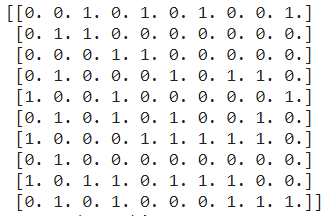
\includegraphics[width=0.5\linewidth]{caso_a}
			\caption{Matriz que representa a melhor configuração para o caso (A)}
			\label{fig:casoa}
		\end{figure}
	\end{frame}

	\begin{frame}
		\frametitle{Caso A}
		\begin{itemize}
			\item Os seguintes dados foram obtidos:
		\end{itemize}
		\begin{table}[H]
			\centering
			\begin{tabular}{|c|c|}
				\hline
				Número de aerogeradores & 37 \\
				\hline
				Custo (\$) & 25,80577 \\
				\hline
				Potência Total (W) & 14590,51096 \\
				\hline
				Valor da função objetivo &  0,001768668\\
				\hline
			\end{tabular}
			\caption{Dados obtidos para o caso (A)}
			\label{tab:casoa}
		\end{table}	
	\end{frame}
	
	\subsection{Caso B}
	\begin{frame}
		\frametitle{Caso B}
		\begin{itemize}
			\item Considera-se que a direção do vento é de $ k = 45^{\circ} $, de Noroeste para Sudeste, e única, portanto $ f_k = 1 $
			\item Obteve-se, assim, a seguinte matriz que representa a configuração do parque eólico:
		\end{itemize}
		\begin{figure}[H]
			\centering
			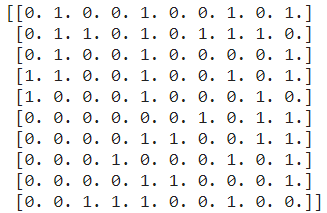
\includegraphics[width=0.5\linewidth]{caso_b}
			\caption{Matriz que representa a melhor configuração para o caso (B)}
			\label{fig:casob}
		\end{figure}
	\end{frame}

	\begin{frame}
		\frametitle{Caso B}
		\begin{itemize}
			\item Os seguintes dados foram obtidos:
		\end{itemize}
		\begin{table}[H]
			\centering
			\begin{tabular}{|c|c|}
				\hline
				Número de aerogeradores &  38\\
				\hline
				Custo (\$) &  26,36009\\
				\hline
				Potência Total (W) &  15824,13293\\
				\hline
				Valor da função objetivo &  0,001665816\\
				\hline
			\end{tabular}
			\caption{Dados obtidos para o caso (B)}
			\label{tab:casob}
		\end{table}	
	\end{frame}

	\subsection{Caso C}
	\begin{frame}
		\frametitle{Caso C}
		\begin{itemize}
			\item Considera-se que a direção do vento é de $ k = 90^{\circ} $,  Oeste para Leste, e também de $ k =  315^{\circ} $, Nordeste para Sudoeste. Para cada caso, considera-se $ f_k = 1 $.
			\item Obteve-se, assim, a seguinte matriz que representa a configuração do parque eólico para $ k = 90^{\circ} $:
		\end{itemize}
		\begin{figure}[H]
			\centering
			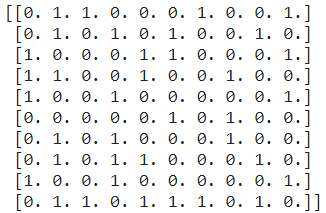
\includegraphics[width=0.5\linewidth]{caso_c_90}
			\caption{Matriz que representa a melhor configuração para o caso (C), com $ k = 90^{\circ} $}
			\label{fig:casoc90}
		\end{figure}
	\end{frame}

	\begin{frame}
		\frametitle{Caso C}
		\begin{itemize}
			\item E para $ k = 315^{\circ} $:
		\end{itemize}
		\begin{figure}[H]
			\centering
			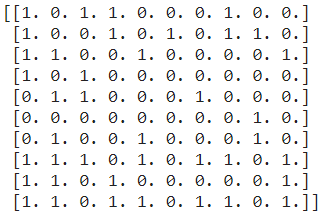
\includegraphics[width=0.5\linewidth]{caso_c_315}
			\caption{Matriz que representa a melhor configuração para o caso (C), com $ k = 315^{\circ} $}
			\label{fig:casoc315}
		\end{figure}
	\end{frame}
	
	\begin{frame}
		\frametitle{Caso C}
		\begin{itemize}
			\item Os seguintes dados foram obtidos, considerando $ k = 90^{\circ} $:
		\end{itemize}
		\begin{table}[H]
			\centering
			\begin{tabular}{|c|c|}
				\hline
				Número de aerogeradores & 37 \\
				\hline
				Custo (\$) & 25,80577 \\
				\hline
				Potência Total (W) & 14761,88185 \\
				\hline
				Valor da função objetivo & 0,001748135 \\
				\hline
			\end{tabular}
			\caption{Dados obtidos para o caso (C), com $ k = 90^{\circ} $}
			\label{tab:casoc90}
		\end{table}	
	\end{frame}

	\begin{frame}
		\frametitle{Caso C}
		\begin{itemize}
			\item E $ k = 315^{\circ} $:
		\end{itemize}
		\begin{table}[H]
			\centering
			\begin{tabular}{|c|c|}
				\hline
				Número de aerogeradores & 40 \\
				\hline
				Custo (\$) & 27,49054 \\
				\hline
				Potência Total (W) & 16688,35799 \\
				\hline
				Valor da função objetivo & 0,001647288 \\
				\hline
			\end{tabular}
			\caption{Dados obtidos para o caso (C), com $ k = 315^{\circ} $}
			\label{tab:casoc315}
		\end{table}	
	\end{frame}

	\subsection{Caso D}
	\begin{frame}
		\frametitle{Caso D}
		\begin{itemize}
			\item Nesse caso, considera-se vários sentidos de incidência dos ventos (0º, 45º, 90º, 135º, 180º, 225º, 270º, 315º), portanto, $ f_k = \dfrac{1}{8} $.
			\item Obteve-se, assim, a seguinte matriz que representa a configuração do parque eólico:
		\end{itemize}
		\begin{figure}[H]
			\centering
			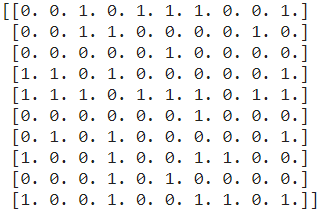
\includegraphics[width=0.5\linewidth]{caso_d}
			\caption{Matriz que representa a melhor configuração para o caso (D)}
			\label{fig:casod}
		\end{figure}
	\end{frame}
	
	\begin{frame}
		\frametitle{Caso D}
		\begin{itemize}
			\item Os seguintes dados foram obtidos:
		\end{itemize}
			\begin{table}[H]
			\centering
			\begin{tabular}{|c|c|}
				\hline
				Número de aerogeradores & 36 \\
				\hline
				Custo (\$) & 25,25843 \\
				\hline
				Potência Total (W) & 14562,36303 \\
				\hline
				Valor da função objetivo & 0,001734500 \\
				\hline
			\end{tabular}
			\caption{Dados obtidos para o caso (D)}
			\label{tab:casod}
		\end{table}	
	\end{frame}
	
	\section{Conclusão}
	\begin{frame}
		\frametitle{Conclusão}
		\begin{itemize}
			\item Pode-se dizer que o COA apresentou eficiência satisfatória, retornando configurações dentro do esperado para todas as direções de vento.
			\item  É perceptível que nos casos (B) e (C) (para $ k = 315^{\circ} $) o coiote alfa encontrado foi melhor adaptado que nos demais casos, mas essa tendência é também vista em \cite{FredericoFerreiraPanoeiro2018}, onde se utiliza de outra metaheurística.
			\item Ademais, os resultados obtidos são compatíveis com o encontrado na literatura \cite{FredericoFerreiraPanoeiro2018} para um estudo de caso semelhante ao utilizado nesse trabalho.
		\end{itemize}
	\end{frame}

	\begin{frame}[allowframebreaks]
		\frametitle{Referências Bibliográficas}
		\printbibliography[
		title={REFERÊNCIAS BIBLIOGRÁFICAS}
		]
	\end{frame}
\end{document}